\documentclass[10pt]{beamer}

\usetheme[progressbar=frametitle]{metropolis}

\usepackage[utf8]{inputenc}
\usepackage[T1]{fontenc}
\usepackage[francais]{babel}
\usepackage{lmodern}
\usepackage{amsmath}
\usepackage{amssymb}
\usepackage{mathrsfs}
\usepackage{appendixnumberbeamer}
\usepackage{subcaption}
\usepackage{booktabs}
\usepackage[scale=2]{ccicons}
\usepackage{pgfplots}
\usepackage{graphicx}
\usepackage{epstopdf}
\usepackage{calrsfs}
\usepackage{mathtools}
\usepackage{xspace}
\usepackage{array,multirow}
\usepackage{amsmath,bm}
\usepackage[cal=boondoxo, calscaled=1.2]{mathalfa}
\usepackage{empheq}
\usepackage[most]{tcolorbox}
\usepackage{url}

\definecolor{vipw}{RGB}{46, 204, 113}

\newcommand{\vip}[1]{\textbf{\textcolor{vipw}{#1}}}

% Box for math equation
\newtcbox{\math1}[1][]{%
    nobeforeafter, math upper, tcbox raise base,
    enhanced, colframe=black!30!black,
    colback=black!30, boxrule=1pt,
    #1}


\usepgfplotslibrary{dateplot}
\pgfplotsset{compat=newest}


% Some minor options 
\definecolor{Purple}{HTML}{3498db}
\definecolor{Orange}{HTML}{CF4A30}

\setbeamercolor{alerted text}{fg=Orange}
\setbeamercolor{frametitle}{bg=Purple}
\setbeamercolor{progress bar}{bg=Purple}
\setbeamercolor{title separator}{bg=Purple}
\setbeamercolor{progress bar in head/foot}{bg=Purple}
\setbeamercolor{progress bar in section page}{bg=Purple}

% Title and co
\title{Contrôle d'un agent par apprentissage par renforcement profond}
\subtitle{Présentation de mon stage à THALES dans l'équipe AS\&BSIM}
\date{\today}
\author{Nizam Makdoud}
\institute{THALES}


\begin{document}
\maketitle

\begin{frame}
    \tableofcontents
\end{frame}


\begin{frame}
\textbf{Sujet du stage}
coucou
\end{frame}


% simple alias for easier change in the future if needed
\newcommand{\mf}[1]{\mathcal{#1}}

\section{Apprentissage Profond}
\begin{frame}{Théorie de l'apprentissage profond}
Formalisme \textbf{La théorie des processus décisionnels de Markov}:
\[
    \bm{\mf{M} = \bigg\{\mf{X}, \mf{A}, \mf{R}, \mf{P}, \gamma\bigg\} }
\]

\begin{center}
    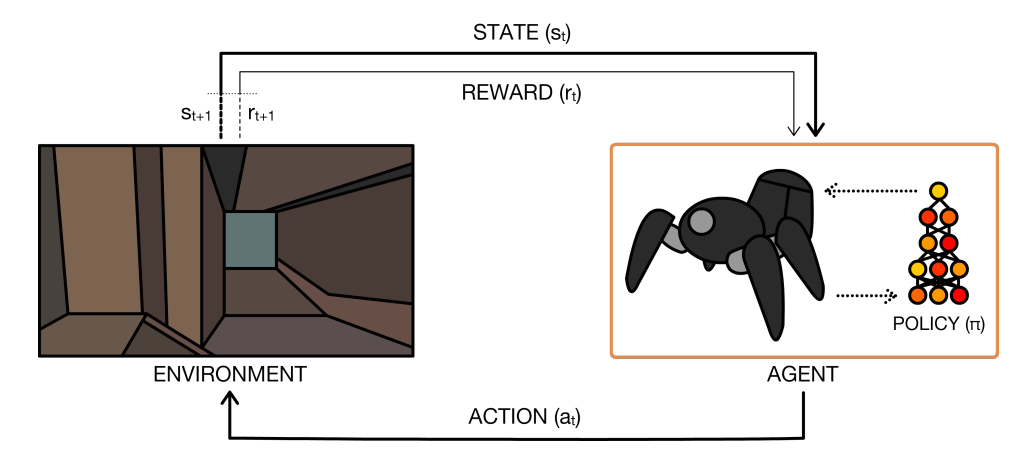
\includegraphics[scale=.2]{./reinforcementlearning/rl}
\end{center}

\end{frame}


\begin{frame}{Théorie de l'apprentissage profond}
Formalisme \textbf{La théorie des processus décisionnels de Markov}:
\[
    \bm{\mf{M} = \bigg\{\mf{X}, \mf{A}, \mf{R}, \mf{P}, \gamma\bigg\} }
\]

\begin{columns}[T] % align columns
\begin{column}{.48\textwidth}
\begin{center}
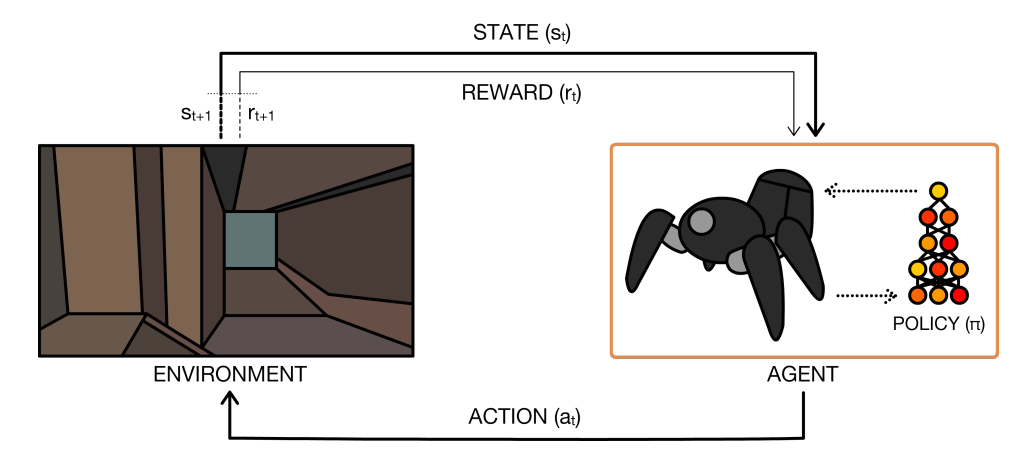
\includegraphics[scale=.14]{./reinforcementlearning/rl}
\end{center}
\end{column}%
\hfill%
\begin{column}{.68\textwidth}
\begin{itemize}
    \item \vip{Politique}\\ $\bm{\pi}$,  $\bm{a_t\:\sim\: \pi\big(\cdot, x_t\big) }$
    \item \vip{Dynamique}\\ $ x_{t+1} \:\sim\: P(\cdot, x_t, a_t) $
    \item \vip{Fonction Etat-Action}\\ $ Q^\pi(x, a) = \underset{P, \pi}{\mathbb{E}} \Big[ \underset{t}{\sum} \gamma^t r_t(x_t, a_t) \,\vert\, x_0,a_0=x,a \Big]$
\end{itemize}
\end{column}%
\end{columns}

\end{frame}

\section{Architecture classique en apprentissage profond}

\begin{frame}
\textbf{Architecture classique en apprentissage profond}
\begin{center}
    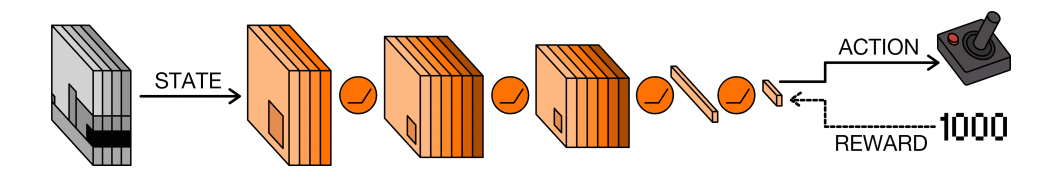
\includegraphics[scale=.3]{./architecturevanilla/vanilla.png}
\end{center}
\end{frame}

\begin{frame}
    \textbf{Gestion des entrées}
\begin{center}
    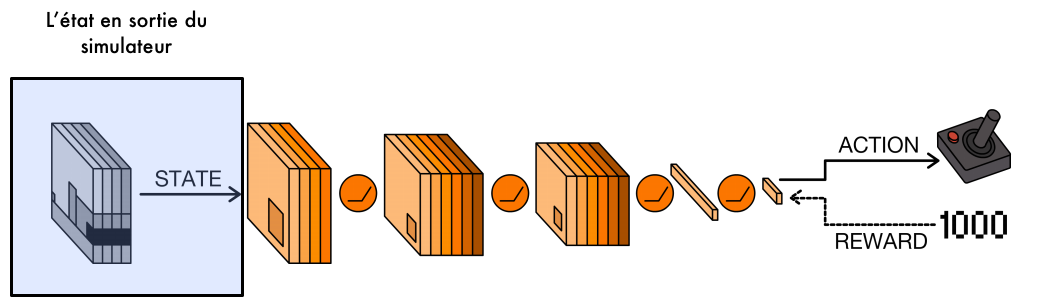
\includegraphics[scale=.3]{./architecturevanilla/stage-0.png}
\end{center}
\end{frame}


\begin{frame}
    \textbf{Acquisitions automatiques d'éléments pertinants à la prise de décisions}
\begin{center}
    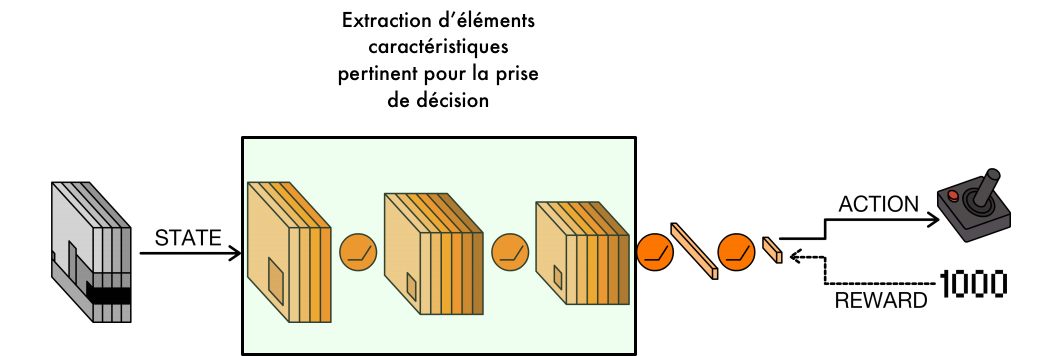
\includegraphics[scale=.3]{./architecturevanilla/stage-1.png}
\end{center}
\end{frame}


\begin{frame}
    \textbf{Prise de la décision par l'agent}
\begin{center}
    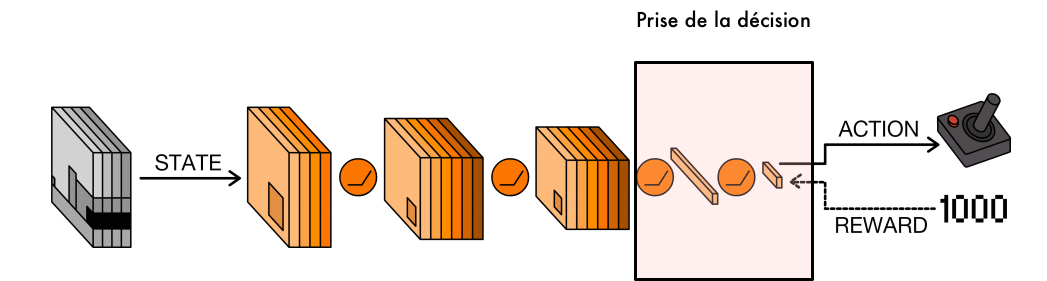
\includegraphics[scale=.3]{./architecturevanilla/stage-2.png}
\end{center}
\end{frame}

\begin{frame}
    \textbf{Apprentissage du réseau}
\begin{center}
    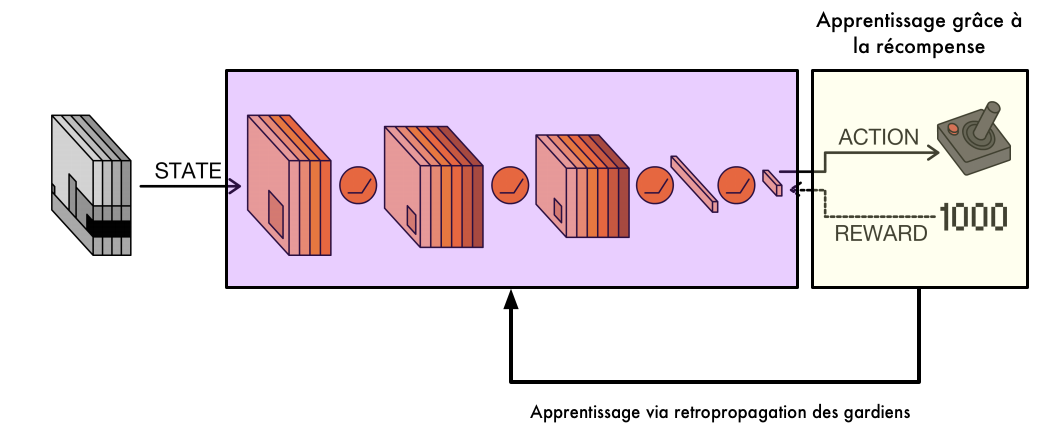
\includegraphics[scale=.3]{./architecturevanilla/stage-3.png}
\end{center}
\end{frame}


\begin{frame}
    \textbf{Résumé de la base utilisée pour le contrôle}
\begin{center}
    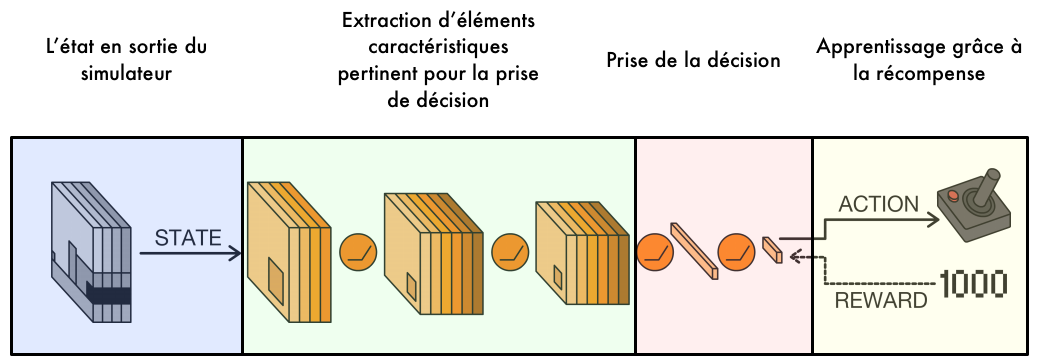
\includegraphics[scale=.3]{./architecturevanilla/stage-4.png}
\end{center}
\end{frame}





\section{Module de curiosité appliqué au contrôle}
\begin{frame}{Nécessité d'exploration d'un environnement}

    Nécessité d'exploration de l'environnement ?

\begin{columns}[T] % align columns
\begin{column}{.48\textwidth}
\begin{center}
    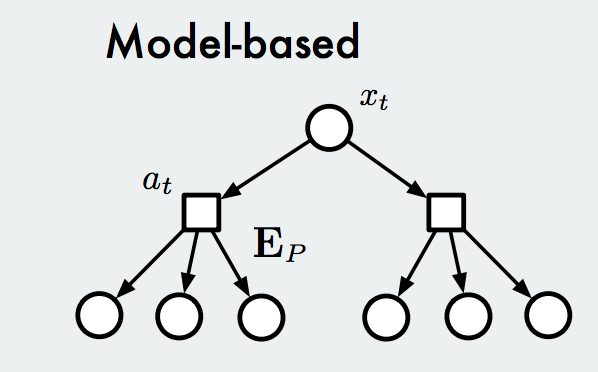
\includegraphics[scale=.24]{./curiosity/1}
\end{center}
\end{column}%
\hfill%
\begin{column}{.58\textwidth}
\begin{itemize}
    \item \vip{Dynamique de l'environnement}\\$\rightarrow$ Connue \\ $\rightarrow$ Fonction d'état-action: Connue \\ $\rightarrow$ Politique: Connue
\end{itemize}

\begin{center}
    \bigskip
    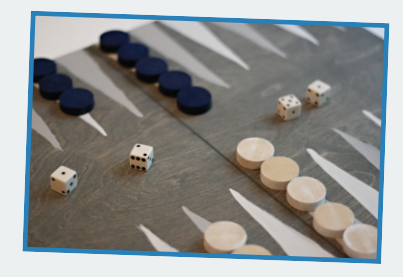
\includegraphics[scale=.3]{./curiosity/3}
\end{center}

\end{column}%
\end{columns}


\end{frame}

\begin{frame}{Nécessité d'exploration d'un environnement}

    Nécessité d'exploration de l'environnement ?

\begin{columns}[T] % align columns
\begin{column}{.48\textwidth}
\begin{center}
    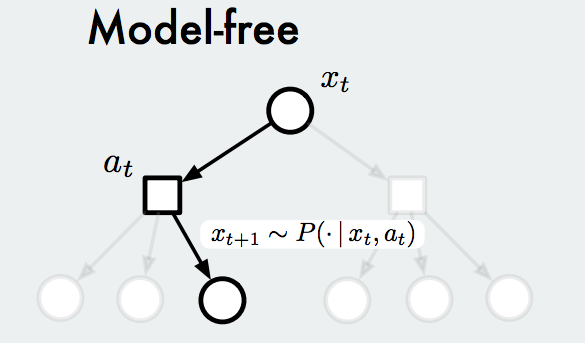
\includegraphics[scale=.24]{./curiosity/2}
\end{center}
\end{column}%
\hfill%
\begin{column}{.58\textwidth}
\begin{itemize}
    \item \vip{Dynamique de l'environnement}\\$\rightarrow$ Inconnue \\ $\rightarrow\:$ Fonction d'état-action: Inconnue \\ $\rightarrow\:$ Politique: Inconnue
\end{itemize}

\bigskip

\begin{center}
    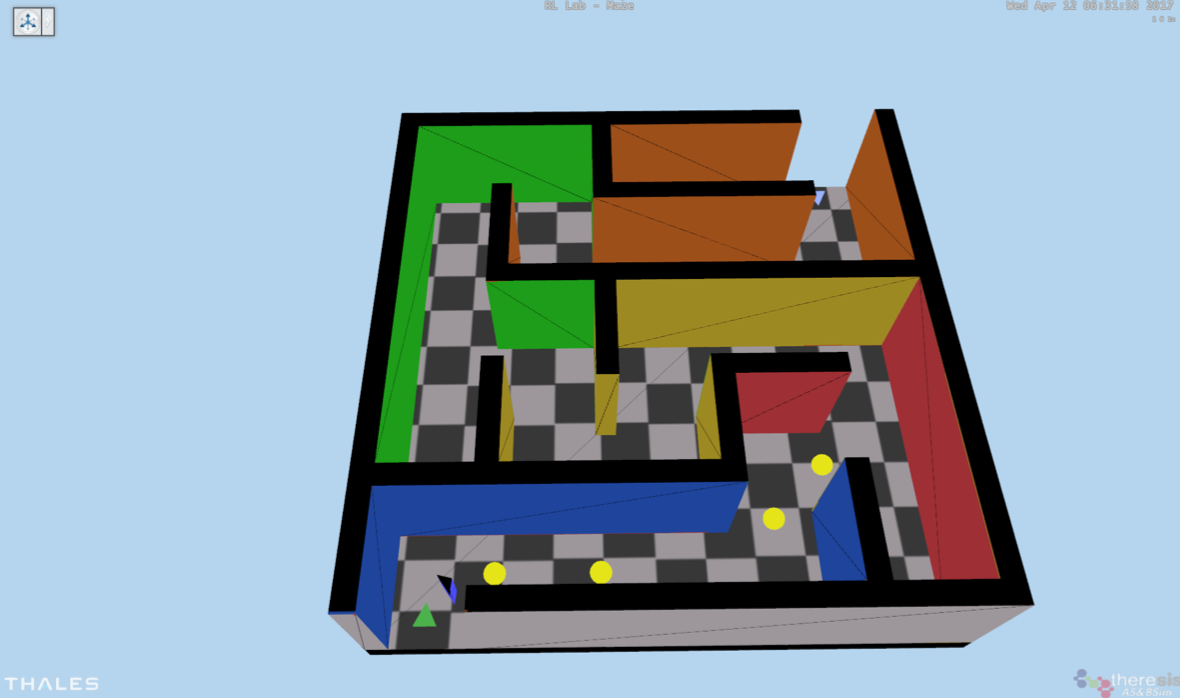
\includegraphics[scale=.1]{./curiosity/4}
\end{center}

\end{column}%
\end{columns}


\end{frame}

\end{document}
